\documentclass[12pt, letterpaper]{article}
\usepackage[utf8]{inputenc}
\usepackage{graphicx} 
\usepackage{textcomp}
\usepackage{gensymb}
\usepackage[shortlabels]{enumitem}
\usepackage{physics}
\usepackage{amssymb}

\title{Axis Transformation\\ \large for the NOVA flight computer data generation suite}
\author{Paul Conway}

\begin{document}
\maketitle
\pagebreak

% Introduction
\begin{center}
\textbf{Introduction}
\end{center}
One of the challenges faced by the NOVA Ground Station is the fact that the flight computer is reporting data from its frame of reference. We will refer to this reference frame as the Vehicle Centered Non-inertial frame, or VCN frame. To make the data more useful, it is important to convert the data from the VCN frame to the frame of reference of the ground station. We will refer to this reference frame as the Ground Station Inertial frame, or GSI frame. Let us examine these two reference frames more closely.
\begin{center}
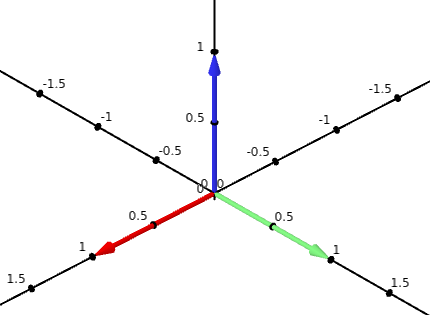
\includegraphics[scale=0.65]{GSI_frame_solo}
\end{center}
In the image above, you can see three vectors. The red, green, and blue vectors are the $\hat{i}$, $\hat{j}$, and $\hat{k}$ unit vectors of the GSI frame. We will color the axes corresponding to each unit vector accoringly. Before the vehicle is launched, it rests on the ground such that the VCN frame aligns with the GSI frame.
\begin{center}
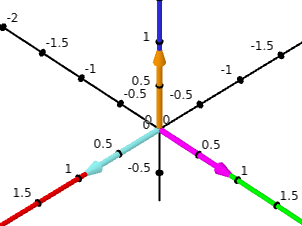
\includegraphics[scale=0.65]{GSI_VCN_aligned}
\end{center}
In the image above, the $\hat{i}_V$, $\hat{j}_V$, and $\hat{k}_V$ vectors have been colored cyan, magenta, and orange respectively. Clearly in this state, transitioning from the VCN to the GSI frame is trival as there is no change to the vectors. Obviously though, this will change. To understand how to make that transition, we have to understand the changes taking place between the two frames. There are in fact two types of changes that can occur between these reference frames: translation and rotation. However, we are only concerned with rotation. \textit{Translational changes do not affect the transition from one frame to another}. This is important to understand as we will treat both frames as sharing the same origin. In reality of course the vehicle is somewhere other than the ground station.
\pagebreak

\begin{center}
\textbf{Rotation Matricies}
\end{center}
\begin{center}
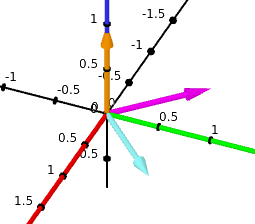
\includegraphics[scale=0.75]{VCN_rot}
\end{center}
In the image above, we can see that the VCN frame has been rotated with respect to the GSI frame. Let us define these rotations more rigorously. \\
Let's begin with what an extrinsic rotation is. An extrinsic rotation is one about a fixed set of axes. In our case, our fixed axes are those defined by GSI frame. The rotation depicted above is an extrinsic rotation. The other type of rotation is an intrisic rotation, which is one about the rotating axes. If we were to rotate the VCN frame about itself, that would be an intrisic rotation. Next we will properly define each rotation.
\begin{itemize}
\item $\alpha$ represents the rotation about the $\hat{i}$ vector
\item $\beta$ represents the rotation about the $\hat{j}$ vector
\item $\gamma$ represents the rotation about the $\hat{k}$ vector
\end{itemize}
Together these angles are refered to as Euler angles, and represent the pitch, yaw, and roll of our system respectively.
Next we will discuss rotation matricies. We know we can express a vector as a matrix. For now, accept that this vector must be represented as a column vector. For example, a vector $\vec{a} = a_x\hat{i} + a_y\hat{j} + a_z\hat{k}$ can be represented as:
\[ \textbf{A} = 
\begin{bmatrix}
r_x \\ r_y \\ r_z
\end{bmatrix}
\]
We can of course rotate this vector. Without getting too much into the linear algebra, for now just understand that we can accomplish this rotation by multiplying our vector by a rotation matrix. For principal axes $xyz$, these matricies are:
\[ R_x(\theta) = 
\begin{bmatrix}
1 & 0 & 0 \\
0 & \cos \theta & -\sin \theta \\
0 & \sin \theta & \cos \theta
\end{bmatrix}
\] \[ R_y(\theta) =
\begin{bmatrix}
\cos \theta & 0 & \sin \theta \\
0 & 1 & 0 \\
-\sin \theta & 0 & \cos \theta
\end{bmatrix}
\] \[ R_z(\theta) = 
\begin{bmatrix}
\cos \theta & -\sin \theta & 0 \\
\sin \theta & \cos \theta & 0 \\
0 & 0 & 1
\end{bmatrix}
\]
In our case, $x=\hat{i}$, $y=\hat{j}$, $z=\hat{k}$. These matricies represent a rotation of angle $\theta$ about their respective axis. For example, to rotate our vector $\textbf{A}$ an angle $\phi$ about the $\hat{j}$ axis to obtain a new vector $\textbf{B}$, we would do the following:
\[
\textbf{B} = R_y(\phi)\textbf{A} = 
\begin{bmatrix}
\cos \phi & 0 & \sin \phi \\
0 & 1 & 0 \\
-\sin \phi & 0 & \cos \phi
\end{bmatrix} \begin{bmatrix}
r_x \\ r_y \\ r_z
\end{bmatrix}
\]
The beauty of this system is that it allows us to easily chain multiple rotations together. For example, if we wanted to obtain matrix $\textbf{B}$ by rotating $\textbf{A}$ through angles $a$, $b$, and $c$ around the $\hat{i}$, $\hat{j}$, and $\hat{k}$ vectors (in that order), we would carry out the following calculation:
\[
\textbf{B} = R_x(a)R_y(b)R_z(c)\textbf{A} =
\] \[
\begin{bmatrix}
1 & 0 & 0 \\
0 & \cos a & -\sin a \\
0 & \sin a & \cos a
\end{bmatrix}
\begin{bmatrix}
\cos b & 0 & \sin b \\
0 & 1 & 0 \\
-\sin b & 0 & \cos b
\end{bmatrix}
\begin{bmatrix}
\cos c & -\sin c & 0 \\
\sin c & \cos c & 0 \\
0 & 0 & 1
\end{bmatrix}
\begin{bmatrix}
r_x \\ r_y \\ r_z
\end{bmatrix}
\]
We could also decide on a different order of rotations. For example, we could rotate $\textbf{A}$ around the $\hat{j}$, $\hat{k}$, then $\hat{i}$ and our calculation would look like:
\[
\textbf{B} = R_y(b)R_z(c)R_x(a)\textbf{A}
\]
We can also just as easily reverse this rotation. If we have $\textbf{B}$ and want to return to $\textbf{A}$ from our $\hat{j}$ then $\hat{k}$ then $\hat{i}$ rotation, we would carry out the following calculation:
\[
\textbf{A} = R_x^{-1}(b)R_z^{-1}(c)R_y^{-1}(a)\textbf{B}
\]
You should notice that the order of these applied rotations changed when going in reverse. That is what the next section will discuss.
\pagebreak

\begin{center}
\textbf{Dealing with Noncommunitivity}
\end{center}
I want you to try something. Pick up your phone or another object that has three distinct axes. Hold it out in front of you and rotate it forward, then clockwise. Remember this orientation. Now reorient your phone as it was before you performed those rotations. This time, rotate it clockwise, then forward. You will notice that the orientation is different from the first set of rotations. Why is this? The basic and most consise answer is that \textit{rotations are not communitive}. That is, in general the order in which you perform a set of rotations matters. This fact by the way is why angles can never be expressed as vectors. The communitive property is a fundamental property of elements in a vector space. \\ \\
This noncommunitivity has many implications for us. While we do have a generalized way to rotate a coordinate system with a set of three angles, and reverse those rotations, we have to know the order with which these rotations were applied. We need a way to rotate a coordinate system such that the order of rotations does not matter. 



\textbf{TODO: May Remove}
This noncommunitivity has many implications for us. While we do have a generalized way to rotate a coordinate system with a set of three angles, and reverse those rotations, we have to know the order with which these rotations were applied. In reality, the vehicle is rotating about all axes simultaneously. To better tackle this problem, we should look more closlely at the vehicle itself. Let us recap some facts about the vehicle, and introduce some new ones:
\begin{itemize}
\item The VCN frame is fixed to the body of the vehicle. 
\item The $\hat{k}_V$ vector always points in the direction of forward motion. For rockets, this is the direction that the nose points.
\item The vehicle is constantly reporting 
\end{itemize}

\pagebreak
\begin{center}
\textbf{Glossary of Terms}
\end{center}
\begin{enumerate}
\item VCN frame
\begin{itemize}
\item Vehicle Centered Non-inertial frame.
\item This is the frame of reference of the vehicle itself.
\item It is expressed with the unit vectors $\hat{i}_V$, $\hat{j}_V$, and $\hat{k}_V$ such that \\ $\hat{i}_V \times \hat{j}_V = \hat{k}_V$ completes a right-handed cartesian coordinate system.
\end{itemize}

\item GSI frame
\begin{itemize}
\item Ground Station Inertial frame.
\item This is the frame of reference of the ground station.
\item It is expressed with the unit vectors $\hat{i}$, $\hat{j}$, and $\hat{k}$ such that $\hat{i} \times \hat{j} = \hat{k}$ completes a right-handed cartesian coordinate system.
\end{itemize}
\end{enumerate}

\end{document}